% Schéma avec le filtre RC pour le découplage, fonctionnement, résultat, mesure à l'oscillo
Afin de supprimer la composante DC, il va nous falloir implémenter un filtre. Un filtre permet de choisir quelles fréquences du signal vont pouvoir passer. Ils permettent soit de ne laisser passer que les hautes, que les basses fréquences ou une bande de fréquences.
Dans ce cas-ci, nous voulons supprimer la constante qui correspond à une fréquence de zéro. Il va donc falloir implémenter un filtre passe haut. Ce filtre est réalisé grâce la capacité C1 et la résistance R2. La capacité est un composant qui accumule des charges électriques. C'est pourquoi, il ne peut y avoir que des variations de tensions à ces bornes. Donc la composante DC, qui ne varie pas, ne passe pas à travers la capacité. Le signal AC lui, n'est pas affecté par celle-ci. \\

Le signal filtré est récupéré aux bornes de la résistance. Vous pouvez observer l'effet du filtre grâce à oscilloscope. Placez une sonde avant le filtre et après le filtre pour voir son effet. 

\begin{figure}[!ht]
	\centering
	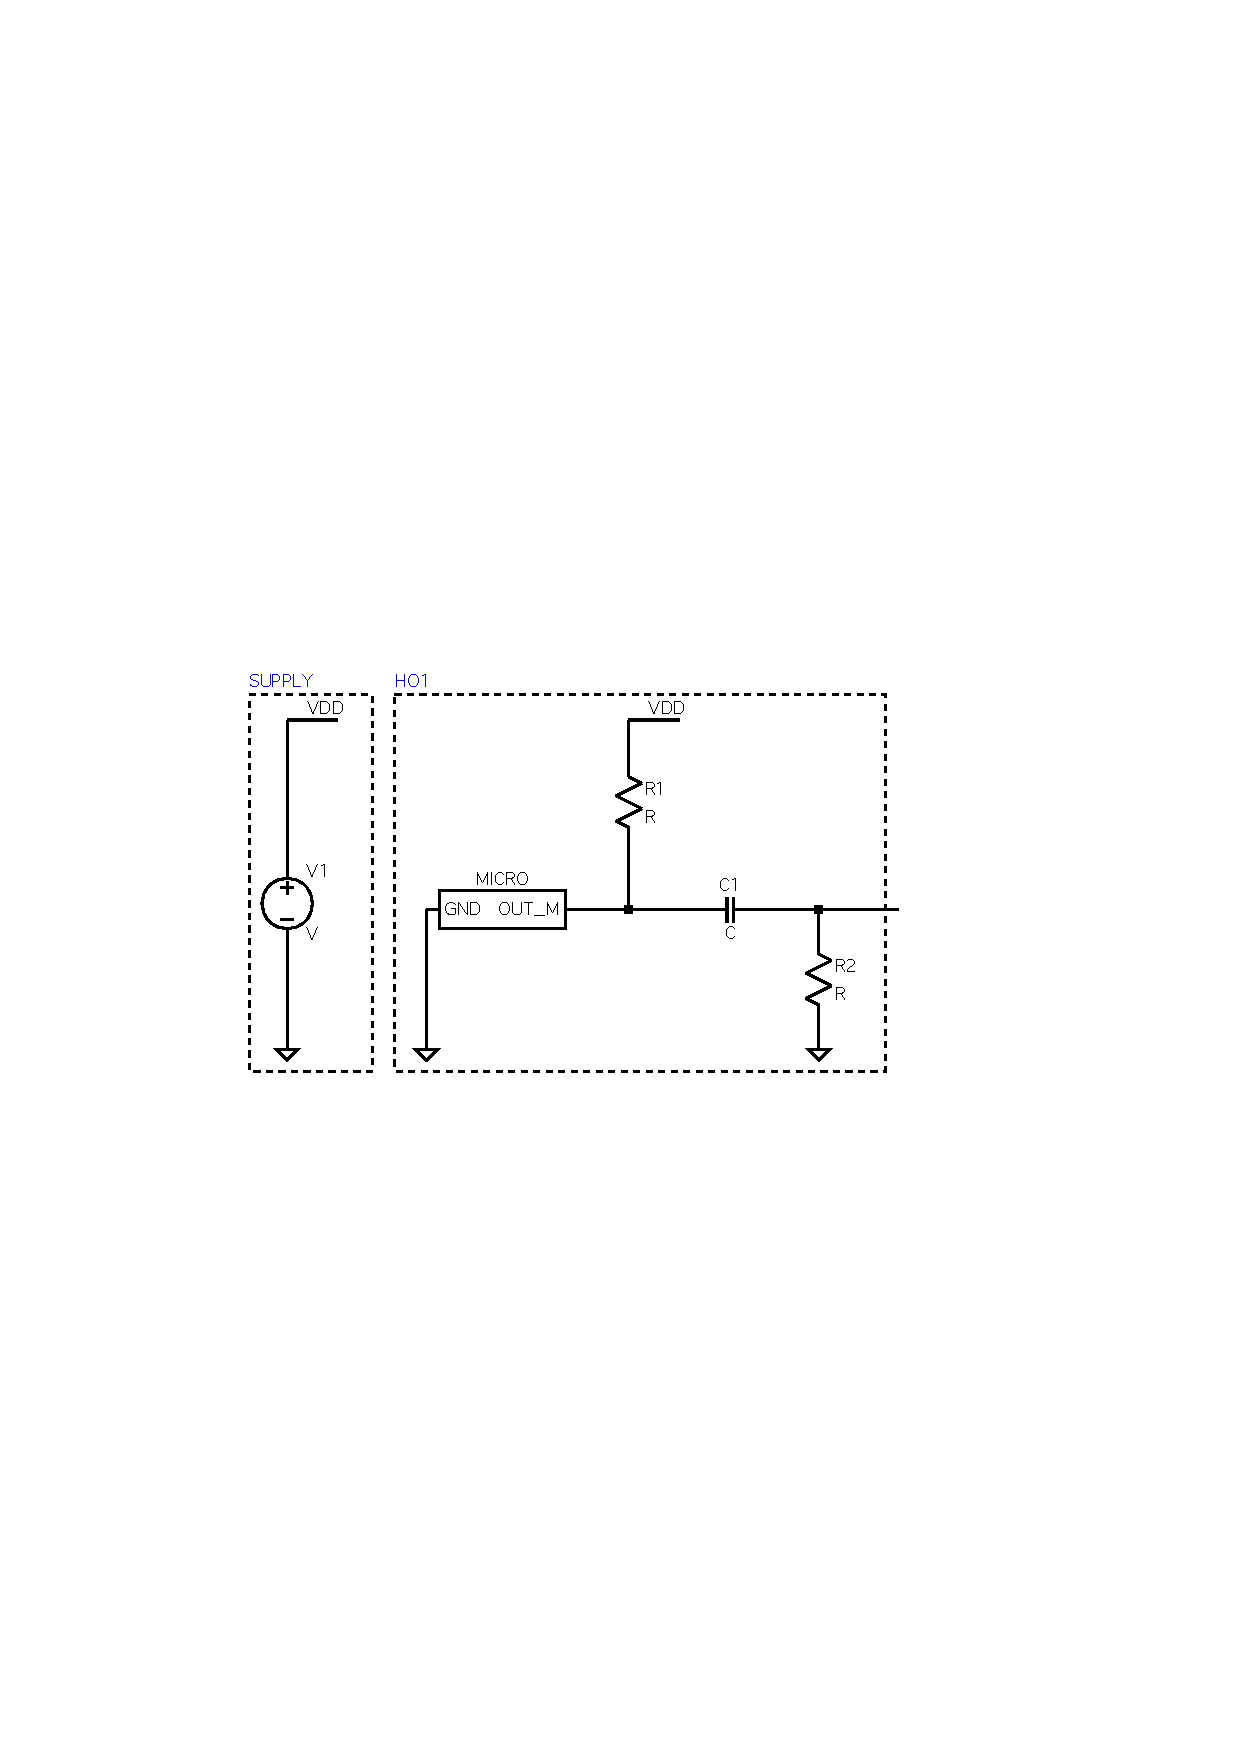
\includegraphics[width=.75\textwidth]{figures/Circuit_P1.pdf}
	\caption{Circuit HO1 avec filtre de découplage. $R2 = 55 k\Omega$, $C1 = 150n F$.}
	\label{fig:circuit_H01_filtre}
\end{figure}
